% =============================================================================
%  Paper 013 — Consent, Disclosure & Participatory Governance for Clinical AI Agents
%  QUOKKAGUARD paper program. House style from papers/_template.
%  Numbers come from numbers.tex (generated by scripts/013-consent/summarize.py);
%  \providecommand defaults below keep the document compilable before a run.
% =============================================================================
\documentclass[11pt]{article}
\usepackage[utf8]{inputenc}
\usepackage[margin=1in]{geometry}
\usepackage{booktabs}
\usepackage{graphicx}
\usepackage{float}
\usepackage{afterpage}
\usepackage[section]{placeins}
\renewcommand{\topfraction}{0.9}
\renewcommand{\bottomfraction}{0.8}
\renewcommand{\textfraction}{0.08}
\renewcommand{\floatpagefraction}{0.75}
\setcounter{topnumber}{3}
\setcounter{bottomnumber}{2}
\setcounter{totalnumber}{5}
\usepackage{amsmath}
\usepackage{amssymb}
\usepackage{hyperref}
\usepackage{xcolor}
\usepackage{listings}
\definecolor{kwblue}{rgb}{0.10,0.20,0.65}
\definecolor{typepurple}{rgb}{0.50,0.15,0.55}
\definecolor{strred}{rgb}{0.62,0.12,0.12}
\definecolor{cmtgreen}{rgb}{0.20,0.45,0.20}
\lstdefinestyle{housespecyaml}{
  basicstyle=\ttfamily\footnotesize,
  backgroundcolor=\color{black!3},
  frame=single,
  framesep=5pt,
  rulecolor=\color{black!45},
  columns=fullflexible,
  breaklines=true,
  keepspaces=true,
  showstringspaces=false,
  alsoletter=_,
  commentstyle=\color{cmtgreen}\itshape,
  stringstyle=\color{strred},
  morecomment=[l]{\#},
  morestring=[b]",
  morestring=[b]',
  keywordstyle=\color{kwblue}\bfseries,
  keywords={patient,status,base,exceptions,kind,purpose,actions,credentials},
  keywordstyle=[2]\color{typepurple}\bfseries,
  keywords=[2]{permit,deny,active,withdrawn,expired,treatment,research,contact,marketing,escalate},
}
\lstdefinestyle{housespecyamlbare}{style=housespecyaml, frame=none,
  backgroundcolor=\color{white}, xleftmargin=0pt, framexleftmargin=0pt,
  aboveskip=1pt, belowskip=0pt}
\usepackage[most]{tcolorbox}
\tcbuselibrary{listings,skins}
\definecolor{cardindigo}{HTML}{4F46E5}
\definecolor{slate}{HTML}{475569}
\definecolor{amber}{HTML}{D97706}
\definecolor{cardblue}{HTML}{1D4ED8}
\definecolor{cardpurple}{HTML}{6D28D9}
\definecolor{cardteal}{HTML}{0F766E}
\tcbset{
  cardcol/.store in=\cardcol, cardcol=cardblue,
  policycard/.style={
    enhanced, breakable=false, arc=3pt, boxrule=0.7pt, top=3pt, bottom=3pt,
    left=7pt, right=7pt, boxsep=1pt, coltitle=white,
    colframe=\cardcol!60!black, colback=white, colbacktitle=\cardcol,
    fonttitle=\bfseries\small, drop fuzzy shadow=black!25,
  },
}
\usepackage{url}
\usepackage{multirow}
\usepackage{array}
\usepackage{ragged2e}
\newcolumntype{L}[1]{>{\RaggedRight\arraybackslash}p{#1}}
\usepackage[htt]{hyphenat}
\hypersetup{colorlinks=true, linkcolor=blue, citecolor=blue, urlcolor=blue}

\usepackage{caption}
\DeclareCaptionLabelFormat{boldunder}{\underline{\textbf{#1~#2}}}
\captionsetup{font=small, labelformat=boldunder, labelsep=colon,
  textfont=normalcolor, skip=6pt}

\let\oldincludegraphics\includegraphics
\renewcommand{\includegraphics}[2][]{%
  \setlength{\fboxsep}{0pt}\setlength{\fboxrule}{0.5pt}%
  \fbox{\oldincludegraphics[#1]{#2}}}

% --- Headline numbers (overridden by numbers.tex) ---------------------------
\providecommand{\EoneModel}{llama3.1:8b}
\providecommand{\EoneN}{120}
\providecommand{\EoneUngatedDisc}{0.0\%}
\providecommand{\EoneGatedDisc}{100.0\%}
\providecommand{\EoneMcnemarFlip}{0}
\providecommand{\EoneMcnemarP}{<0.001}
\providecommand{\EoneViolUngated}{100.0\%}
\providecommand{\EoneViolGated}{0.0\%}
\providecommand{\EoneViolCases}{0}
\providecommand{\EtwoCVP}{100.0\%}
\providecommand{\EtwoFBR}{0.0\%}
\providecommand{\EtwoViolTotal}{0}
\providecommand{\EtwoInscope}{0}
\providecommand{\EthreeBaseCov}{0.0\%}
\providecommand{\EthreeGatedCov}{100.0\%}
\providecommand{\EthreeLatencyUs}{0.00}
\providecommand{\EfourCGP}{100.0\%}
\providecommand{\EfourFriction}{0.0\%}
\providecommand{\EfourShould}{0}
\providecommand{\EfiveTPR}{0.0\%}
\providecommand{\EfiveFPR}{0.0\%}
\providecommand{\EfiveKappa}{0.00}
\providecommand{\EfiveN}{0}
\providecommand{\EsixPerDecisionUs}{0.000}
\providecommand{\EsixThroughput}{0M}
\providecommand{\EsixDecisions}{0}
\IfFileExists{numbers.tex}{% Auto-generated by scripts/013-consent/summarize.py — do not edit.
% Core macros are \providecommand'd in main.tex; override here.
\renewcommand{\EoneModel}{llama3.1:8b}
\renewcommand{\EoneN}{120}
\renewcommand{\EoneUngatedDisc}{0.0\%}
\renewcommand{\EoneGatedDisc}{100.0\%}
\renewcommand{\EoneMcnemarFlip}{120}
\renewcommand{\EoneMcnemarP}{<10^{-4}}
\renewcommand{\EoneViolUngated}{100.0\%}
\renewcommand{\EoneViolGated}{0.0\%}
\renewcommand{\EoneViolCases}{22}
\renewcommand{\EtwoCVP}{100.0\%}
\renewcommand{\EtwoFBR}{0.0\%}
\renewcommand{\EtwoViolTotal}{311}
\renewcommand{\EtwoInscope}{289}
\renewcommand{\EthreeBaseCov}{0.0\%}
\renewcommand{\EthreeGatedCov}{100.0\%}
\renewcommand{\EthreeLatencyUs}{3.79}
\renewcommand{\EfourCGP}{100.0\%}
\renewcommand{\EfourFriction}{0.0\%}
\renewcommand{\EfourShould}{74}
\renewcommand{\EfiveTPR}{98.5\%}
\renewcommand{\EfiveFPR}{0.0\%}
\renewcommand{\EfiveKappa}{0.61}
\renewcommand{\EfiveN}{300}
\renewcommand{\EsixPerDecisionUs}{2.409}
\renewcommand{\EsixThroughput}{0.4M}
\renewcommand{\EsixDecisions}{356{,}000}
}{}

\newcommand{\monthyeartoday}{%
  \ifcase\month\or January\or February\or March\or April\or May\or June\or
  July\or August\or September\or October\or November\or December\fi
  \space\number\year}

\begin{document}

% ============================================================================
\thispagestyle{empty}
\noindent
\begin{minipage}[c]{0.55\textwidth}
  \raggedright\oldincludegraphics[height=1.05cm]{figs/quome.png}
\end{minipage}\hfill
\begin{minipage}[c]{0.4\textwidth}
  \raggedleft\itshape\large \monthyeartoday
\end{minipage}

\vspace{1.1em}
\begin{center}
  {\LARGE\bfseries Consent Is a Gateway Responsibility:\\[2pt]
   Enforcing Patient Consent, AI Disclosure, and Participatory Governance
   for Clinical AI Agents\par}

  \vspace{0.9em}
  {\large
   QUOKKAGUARD Working Group\textsuperscript{1,\,*}\par}

  \vspace{0.7em}
  {\small
   \textsuperscript{1}\,Quome \par}
  \vspace{0.35em}
\end{center}

\vspace{0.5em}
\begin{tcolorbox}[breakable, enhanced jigsaw, colback=black!4, colframe=black!4,
  arc=5pt, boxrule=0pt, left=16pt, right=16pt, top=10pt, bottom=10pt]
\setlength{\parskip}{0pt}
{\centering\large\bfseries Abstract\par}
\smallskip
\fontsize{9.5}{11.3}\selectfont
Security and policy layers can make a clinical AI agent's actions \emph{authorized}
and \emph{clinically correct} and still leave them \emph{unlawful}: an action taken
outside the patient's recorded consent, or a patient-facing message that hides its
AI authorship, is a compliance and ethical violation regardless of clinical merit.
These patient-facing controls --- consent, disclosure, operator competency, and
goals-of-care --- are exactly the ones inline security firewalls do not address. We
introduce \textbf{\texttt{consent}}, an enforcing gateway layer for the QUOKKAGUARD
\texttt{qfire} proxy that runs after agent identity and policy authorization: it
gates each action on a FHIR-Consent-shaped directive, stamps an AI-involvement
disclosure onto patient-facing output, requires a signed credentialed-operator
attestation for credentialed actions, flags actions conflicting with documented
goals-of-care, and anchors participatory-governance inputs to the tamper-evident
audit chain. Our central, honest finding: a live \texttt{\EoneModel{}} gateway
drafting patient messages discloses AI involvement in only \textbf{\EoneUngatedDisc{}}
of cases and has no consent context to stop out-of-scope contact (a violation on
\textbf{\EoneViolUngated{}} of withdrawn/expired/out-of-scope cases); the
\texttt{consent} layer lifts disclosure to \EoneGatedDisc{} (McNemar $p\,\EoneMcnemarP$)
and out-of-scope action to \EoneViolGated{}. Consent-scope gating prevents
\EtwoCVP{} of violations at a \EtwoFBR{} in-scope false-block rate; competency
gating prevents \EfourCGP{} of unqualified credentialed actions at \EfourFriction{}
friction; goals-of-care detection reaches \EfiveTPR{} at \EfiveFPR{} false-block
($\kappa=\EfiveKappa$). The layer adds \EsixPerDecisionUs{}~µs per decision. All
code, the ConsentBench corpus, and result artifacts are released; all data are
synthetic.

\medskip
\noindent\textbf{Keywords:}~informed consent; AI disclosure; FHIR Consent; clinical
AI agents; participatory governance; healthcare AI safety; gateway enforcement.

\medskip
\noindent\textcolor{blue}{\textbf{Framework:}}~implements HAARF control~C4~\cite{schwoebel2026haarf} --- the Healthcare AI Agents Regulatory Framework, the source of the QUOKKAGUARD program.\\
\noindent\textcolor{blue}{\textbf{Code \& data:}}~\href{https://github.com/quome-cloud/quconsent}{\texttt{github.com/quome-cloud/quconsent}}\\
\noindent\textcolor{blue}{\textbf{Correspondence:}}~\href{mailto:research@quome.com}{research@quome.com}
\end{tcolorbox}

\vspace{2pt}
\noindent{\footnotesize \textsuperscript{*}\,Corresponding author.}
\vspace{0.3em}

% ============================================================================
\section{Introduction}
A clinical AI agent can be perfectly behaved by every measure a security firewall
applies --- the prompt is benign, the goal is pristine, the tool call is within
scope and authorized by policy --- and the resulting action can still be a legal and
ethical violation. If the patient never consented to that use of their data, if the
message the agent sends never says it was written by an AI, if the order requires a
credentialed human who is not in the loop, or if the action cuts against the
patient's documented goals-of-care, then \emph{clinical correctness does not
launder the breach}. These are the patient-facing controls of healthcare
governance, and they are precisely the controls that inline prompt firewalls and
policy engines were never designed to enforce.

The QUOKKAGUARD program builds one security proxy, \texttt{qfire}, one layer at a
time. Prior layers established a pristine goal anchor and tamper-evident provenance,
a policy-as-code authorization band, PHI egress control, multi-agent identity, and
risk-calibrated human oversight. Each makes an action \emph{safer} or \emph{better
authorized}. None asks the orthogonal question this paper asks: \emph{was this
action consented to, disclosed, competently supervised, and aligned with what the
patient said they want?}

\begin{figure}[htb]
\centering
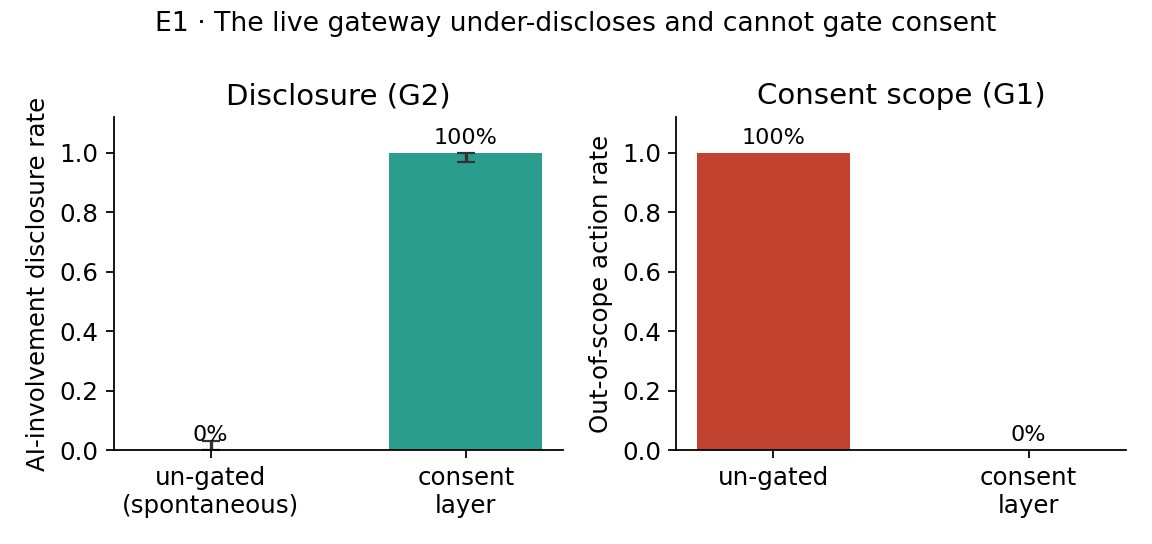
\includegraphics[width=0.95\linewidth]{figs/fig1_live_gap.png}
\caption{\textbf{The paper in one figure.} Run through a live \texttt{\EoneModel{}}
gateway with a neutral clinical-agent prompt, the model drafts clinically-fine
patient messages but volunteers an AI-involvement disclosure in only \EoneUngatedDisc{}
of them \emph{(left)}, and --- having no consent context --- proceeds to contact the
patient even when consent is withdrawn, expired, or out of scope \emph{(right)}. The
\texttt{consent} layer makes disclosure and consent \emph{gateway} responsibilities:
coverage rises to \EoneGatedDisc{} and out-of-scope action falls to \EoneViolGated{}.}
\label{fig:hero}
\end{figure}

We close this gap with \texttt{consent}, a single enforcing layer wired into the
\texttt{qfire} gateway after identity and policy. Its thesis is structural:
\emph{disclosure and consent cannot be left to the model's discretion} --- they must
be enforced at the gateway, where they can be audited. Figure~\ref{fig:hero} is the
evidence: a capable open model, asked to draft patient messages, is warm, clear, and
clinically appropriate, yet it almost never says it is an AI and it has no way to
know the patient withdrew consent. The fix is not a better prompt; it is a control
plane.

\paragraph{Contributions.}
\begin{enumerate}
  \item \textbf{The central result.} On a live \texttt{\EoneModel{}} gateway,
  spontaneous AI-involvement disclosure on patient-facing messages is
  \EoneUngatedDisc{}; the \texttt{consent} layer raises it to \EoneGatedDisc{}
  (McNemar $p\,\EoneMcnemarP{}$) and drives out-of-scope action from
  \EoneViolUngated{} to \EoneViolGated{}.
  \item \textbf{The layer.} \texttt{consent} --- a FHIR-Consent scope gate, an
  output-path disclosure attacher, a signature-verified competency gate, a
  goals-of-care conflict flagger, and a hash-chained participatory-governance
  ledger --- in \textasciitilde1\,kLOC of Rust, adding \EsixPerDecisionUs{}~µs per
  decision.
  \item \textbf{ConsentBench.} A synthetic, deterministic corpus of FHIR-Consent
  directives, scope/competency scenarios with ground truth, patient-facing prompts,
  and scored goals-of-care cases (Apache-2.0).
  \item \textbf{Measured enforcement.} Consent-scope prevention \EtwoCVP{} at
  \EtwoFBR{} false-block; competency prevention \EfourCGP{} at \EfourFriction{}
  friction; goals-of-care detection \EfiveTPR{} at \EfiveFPR{} false-block,
  $\kappa=\EfiveKappa$.
\end{enumerate}

\paragraph{Positioning.} Inline guardrail and firewall systems classify prompts and
responses for safety; policy engines authorize tool calls. \texttt{consent} is
orthogonal to both: it enforces patient-facing legal/ethical obligations that hold
even when safety and authorization pass. It maps to HAARF~\cite{schwoebel2026haarf} controls
C4.1, C4.5, C4.6, C4.9 and C5.6.

% ============================================================================
\section{Problem Setting and Threat Model}
\paragraph{Baseline.} We assume the always-on quanchor baseline: a sealed goal
anchor, a hash-chained provenance ledger, and the upstream enforcement band ---
admission, policy authorization, egress control, agent identity, and human
oversight. The host/operator is untrusted; signing keys are released by
attestation. \texttt{consent} states what it adds \emph{beyond} this baseline.

\paragraph{The five harms.} An action that passes identity and policy can still
realize:
\begin{itemize}
  \item \textbf{G1 Consent-scope violation} --- a data use, contact, treatment, or
  research action outside the patient's recorded consent.
  \item \textbf{G2 Non-disclosure} --- AI involvement in a patient-facing decision
  or message is not disclosed (C4.6).
  \item \textbf{G3 Competency gap} --- a credentialed action is taken with an
  unqualified or absent operator (C4.5, C5.6).
  \item \textbf{G4 Goals-of-care breach} --- an action conflicts with the patient's
  documented values (C4.9).
  \item \textbf{G5 No participatory-governance trail} --- no record that affected
  patients/public had input into the agent's deployment (C4.1).
\end{itemize}
None is a security failure in the usual sense; each is a governance failure that a
clinically-correct, authorized agent can commit. The adversary here is not
necessarily malicious --- it is an ordinary capable model with no consent context
and no obligation, by default, to disclose itself.

\begin{table}[htb]\centering\small
\begin{tabular}{L{3.0cm}L{4.3cm}L{4.3cm}}
\toprule
Layer & What it enforces & What it leaves to \texttt{consent} \\
\midrule
Policy authorization (quwarden) & action allowed in context by role/scope & whether the \emph{patient} consented to it \\
Egress / DLP (qudam) & PHI does not leak on the response path & whether the response \emph{discloses} its AI authorship \\
Identity (quorum) & the agent is who it claims & whether a \emph{credentialed human} stands behind a credentialed act \\
Oversight (qutriage) & ambiguous actions reach a human & which actions are \emph{consent/values} ambiguous in the first place \\
\textbf{This work (quconsent)} & consent, disclosure, competency, goals-of-care, governance & --- \\
\bottomrule
\end{tabular}
\caption{\texttt{consent} enforces the patient-facing obligations the upstream
band does not. Each upstream layer is necessary; none asks whether the patient
agreed, or whether the agent said it was an agent.}
\label{tab:positioning}
\end{table}

% ============================================================================
\section{System Design}
\subsection{Where the layer sits}
\texttt{consent} runs after identity and policy on the request path, with a
disclosure stage on the response path. It composes four request-time controls ---
scope (G1), competency (G3), goals-of-care (G4) --- short-circuiting on the first
that stops the action, plus the output-path disclosure attacher (G2); the
governance ledger (G5) is an out-of-band append-only record. Crucially, an action
in consent \emph{doubt} (withdrawn, expired, missing, or unverified) is never
silently allowed: it is routed to human review (\texttt{Escalate}, handled by the
qutriage oversight layer), while an \emph{explicit} consent denial is a hard
\texttt{Deny}.

\subsection{Consent scope (G1)}
The scope gate resolves each action against a FHIR-Consent-shaped
directive~\cite{fhir_consent}: a
lifecycle \texttt{status}, a default \texttt{base} stance, and purpose-scoped
\texttt{permit}/\texttt{deny} exceptions. Resolution is default-deny with
most-specific-match (an action-level provision overrides a purpose-level one; ties
favour deny). A non-active directive --- withdrawn, expired, or draft --- cannot
authorize anything and escalates.

\begin{figure}[htb]\centering
\begin{tcolorbox}[policycard, cardcol=cardteal, title=A FHIR-Consent directive (ConsentBench), width=0.82\linewidth]
\begin{lstlisting}[style=housespecyamlbare]
patient: pt-0042
status: active
base: deny                 # default-deny
exceptions:
  - { kind: permit, purpose: treatment, actions: [] }
  - { kind: permit, purpose: contact,   actions: [] }
  - { kind: deny,   purpose: treatment, actions: [order_controlled_substance] }
# research/marketing fall through to base=deny -> escalate
\end{lstlisting}
\end{tcolorbox}
\caption{A consent directive as a declarative artifact. Treatment and contact are
permitted; controlled-substance orders are carved out to a hard deny; research and
marketing are not permitted and escalate to human review.}
\label{fig:directive}
\end{figure}

\subsection{Disclosure (G2)}
A complete AI-involvement disclosure must carry three cues: AI/automated authorship,
human-clinician oversight, and a way to reach a human or opt out. A deliberately
simple, auditable detector scores these cues; the output-path attacher stamps a
canonical disclosure onto any patient-facing message lacking one (and never
double-stamps). The detector doubles as the measurement instrument for the live
study (\S\ref{sec:e1}).

\subsection{Competency (G3)}
Credentialed action classes (controlled-substance orders, chemotherapy, final
diagnosis) require a signed \texttt{OperatorAttestation}. The gate verifies an
ed25519 signature over the operator's identity and credential set against the
operator's registered key; an unsigned, mis-signed, missing, or under-credentialed
operator escalates. Forging an attestation or tampering its credential set after
signing fails verification.

\subsection{Goals-of-care (G4)}
Each patient may carry documented values (comfort-focused, DNR, no blood products).
A scored conflict check escalates an action at or above a clinician-tunable
threshold; absent a score, a contraindication map flags actions that contradict a
recorded value. The threshold makes the detection/false-block trade-off an explicit
operating choice (\S\ref{sec:e5}).

\subsection{Participatory-governance ledger (G5)}
An append-only, hash-chained ledger records the participatory-governance inputs that
legitimize a patient-facing deployment --- community reviews, advisory sign-offs,
public-comment summaries --- each entry chained as in the quledger audit log, with the
head hash anchored into that chain. Any retroactive edit, deletion, or reorder
breaks verification. G5 is a mechanism with a tamper-evidence guarantee, not a
hypothesis test.

\subsection{Implementation}
\texttt{consent} is \textasciitilde1\,kLOC of Rust 2021 (\texttt{src/consent/}:
\texttt{engine}, \texttt{disclosure}, \texttt{competency}, \texttt{goals},
\texttt{ledger}, \texttt{metrics}, \texttt{reporter}), reusing the ed25519 plumbing
from the identity layer and the SHA-256 chaining from the audit log. Every decision
is serialized to the tamper-evident audit chain. The layer adds no heavy
dependencies.

% ============================================================================
\section{Experimental Setup}
\paragraph{ConsentBench.} A deterministic (seed~42), synthetic corpus under
\texttt{datasets/013-consent/}: 200 FHIR-Consent directives; 712 scope/competency
scenarios each with a ground-truth expected gateway behavior and family tag; 120
patient-facing prompts tagged with consent status; and 300 scored goals-of-care
cases with clinician-style labels. No PHI; identifiers are synthetic.

\paragraph{Live gateway.} E1 runs each patient-facing prompt through the real
\texttt{qfire} gateway against a local Ollama \texttt{\EoneModel{}} (no paid keys),
under a neutral clinical-agent system prompt that is \emph{silent about disclosure}
so we measure the model's spontaneous behavior. The remaining experiments are
deterministic.

\paragraph{Metrics \& statistics.} Rate metrics carry 95\% Wilson
intervals~\cite{wilson1927}; the paired un-gated-vs-gated disclosure comparison uses
McNemar's test~\cite{mcnemar1947} (exact for $<25$ discordant pairs,
continuity-corrected $\chi^2$ otherwise); goals-of-care label agreement uses
Cohen's $\kappa$~\cite{cohen1960} over two synthetic clinician raters (ground truth
plus fixed-schedule noise). Model snapshot and seed are pinned. A FHIR/Synthea
cross-check~\cite{synthea2018} against real consent structures is future work.

% ============================================================================
\section{Results}\label{sec:results}
\subsection{The live disclosure and consent gap (E1)}\label{sec:e1}
On \EoneN{} patient-facing prompts, the un-gated gateway draws clinically-appropriate
messages but volunteers an AI-involvement disclosure in only \EoneUngatedDisc{} of
them (Figure~\ref{fig:hero}, left). Because the gateway carries no consent context,
it produces a message on every one of the \EoneViolCases{} cases whose consent state
forbids contact --- an out-of-scope action rate of \EoneViolUngated{}. With the
\texttt{consent} layer, the output-path attacher lifts disclosure coverage to
\EoneGatedDisc{} (\EoneMcnemarFlip{} discordant pairs, all in the
undisclosed$\rightarrow$disclosed direction; McNemar $p\,\EoneMcnemarP{}$), and the
scope gate escalates every out-of-scope case, cutting the violation rate to
\EoneViolGated{}. We read this not as a model indictment but as a structural claim:
\emph{disclosure and consent are gateway responsibilities a capable model does not
discharge on its own}. This holds at the frontier: re-running E1 with
\texttt{gpt-oss:120b} (a 117B-parameter Mixture-of-Experts model) reproduces the gap
exactly --- spontaneous disclosure $0\%$, out-of-scope action $100\%$, both driven to
$100\%$ and $0\%$ respectively by the \texttt{consent} layer (McNemar
$p<10^{-26}$) --- so the responsibility gap is structural, not an artifact of an
under-capable model.

\subsection{Consent-scope enforcement (E2)}
\begin{figure}[htb]
\centering
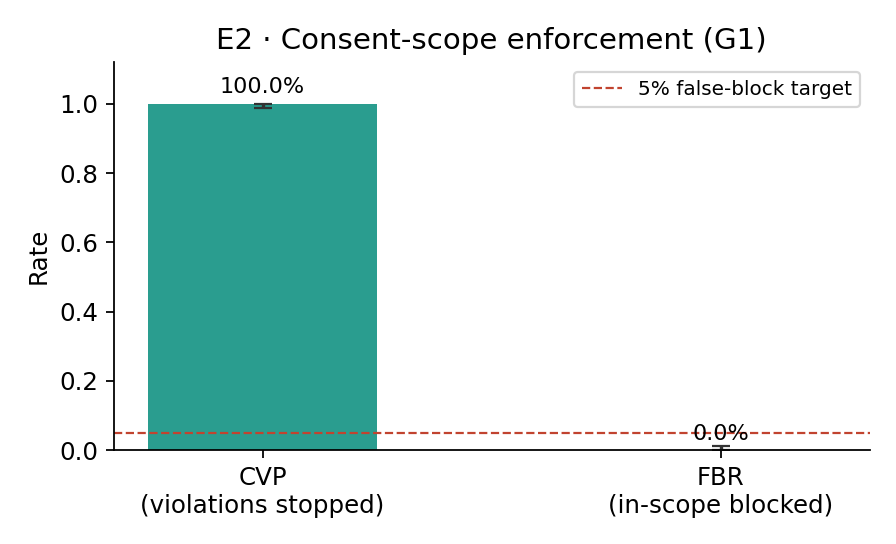
\includegraphics[width=0.62\linewidth]{figs/fig2_enforcement.png}
\caption{\textbf{Consent-scope enforcement (G1).} Across \EtwoViolTotal{} violation
cases (out-of-scope, explicit-deny, withdrawn, expired, draft) the scope gate
prevents \EtwoCVP{}; across \EtwoInscope{} in-scope cases it wrongly blocks
\EtwoFBR{}.}
\label{fig:e2}
\end{figure}
The FHIR-Consent scope gate prevents \EtwoCVP{} of G1 violations at a \EtwoFBR{}
in-scope false-block rate (Figure~\ref{fig:e2}). The result is by construction in
the sense that the gate's resolution \emph{is} the consent semantics --- which is
the point: once consent is machine-readable, enforcement is exact, and the
remaining hard cases (withdrawn/expired/missing) are routed to humans rather than
guessed.

\subsection{Disclosure coverage (E3)}
Bare patient-facing outputs disclose AI involvement \EthreeBaseCov{} of the time; the
attacher raises coverage to \EthreeGatedCov{} at \EthreeLatencyUs{}~µs per message,
and never double-stamps an already-disclosed message.

\subsection{Competency gating (E4)}
\begin{figure}[htb]
\centering
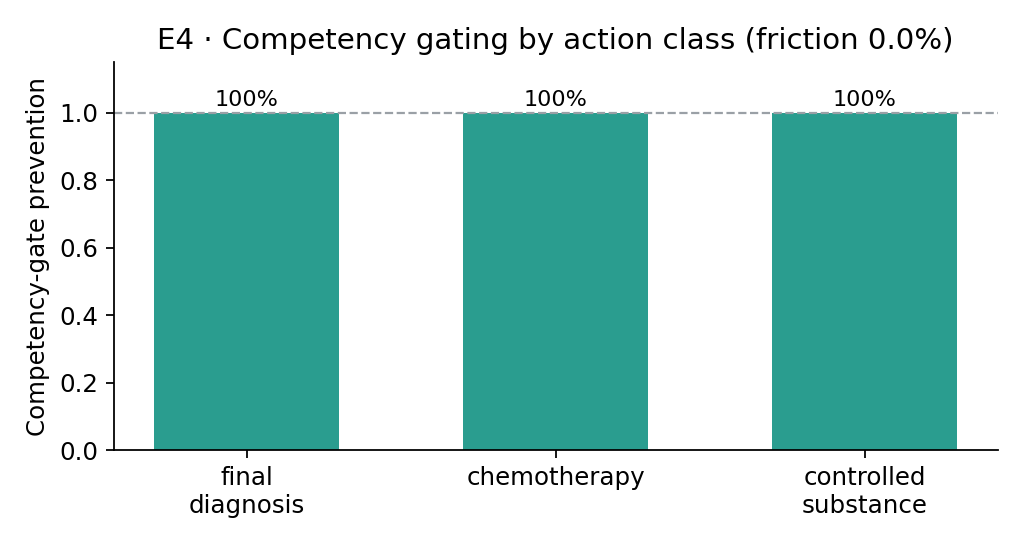
\includegraphics[width=0.70\linewidth]{figs/fig4_competency.png}
\caption{\textbf{Competency gating (G3).} Across \EfourShould{} cases that should be
stopped (missing, uncredentialed, or forged operator), the signature-verified gate
prevents \EfourCGP{} for every credentialed action class, at \EfourFriction{}
friction on validly-credentialed actions.}
\label{fig:e4}
\end{figure}
The competency gate prevents \EfourCGP{} of unqualified credentialed actions ---
including forged attestations and post-signing credential tampering, which fail
ed25519 verification --- at \EfourFriction{} friction on legitimately credentialed
operators (Figure~\ref{fig:e4}).

\subsection{Goals-of-care detection (E5)}\label{sec:e5}
\begin{figure}[htb]
\centering
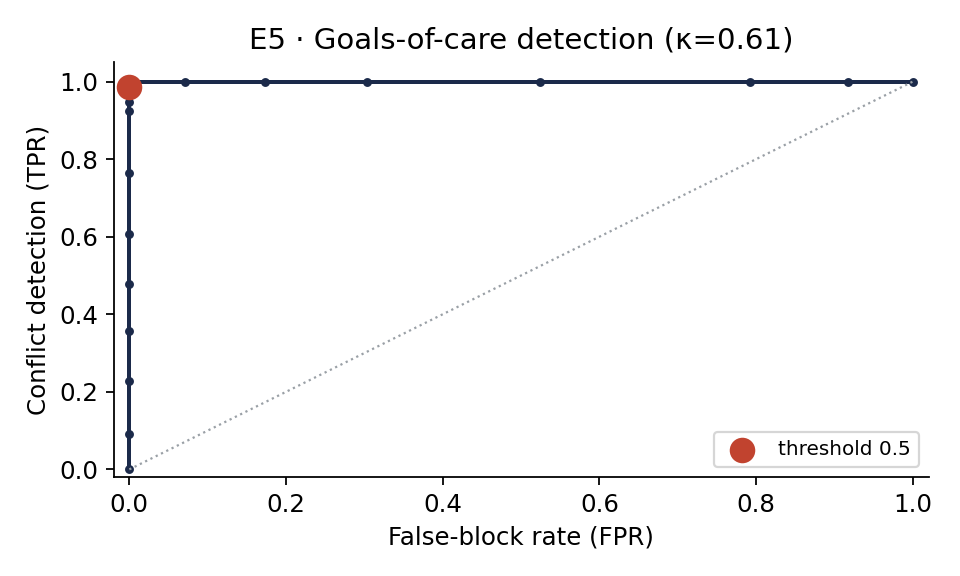
\includegraphics[width=0.60\linewidth]{figs/fig5_goals.png}
\caption{\textbf{Goals-of-care detection (G4).} The threshold sweep traces the
detection/false-block trade-off over \EfiveN{} scored cases; at the default
threshold the gate reaches \EfiveTPR{} detection at \EfiveFPR{} false-block.
Inter-rater agreement on the conflict labels is $\kappa=\EfiveKappa$.}
\label{fig:e5}
\end{figure}
Unlike consent scope, goals-of-care conflict is a graded judgment. The sweep
(Figure~\ref{fig:e5}) makes the trade-off explicit; at the default threshold the
gate catches \EfiveTPR{} of conflicts at \EfiveFPR{} false-block. The
moderate-to-substantial inter-rater agreement ($\kappa=\EfiveKappa$) is itself the
honest caveat: values conflicts are not crisp, which is exactly why flagged cases
escalate to a clinician rather than being auto-denied.

\subsection{Overhead (E6)}
Over \EsixDecisions{} decisions the full layer (scope + goals-of-care + disclosure)
costs \EsixPerDecisionUs{}~µs per decision (\EsixThroughput{} decisions/s),
negligible against any LLM call.

% ============================================================================
\section{Discussion and Limitations}
\paragraph{Interpretation.} The recurring shape of these results is that the
\emph{crisp} obligations --- is there an active permitting provision? is there a
valid credential signature? --- enforce exactly and cheaply once represented
machine-readably, while the \emph{graded} obligations --- does this message
disclose enough? does this action betray the patient's goals? --- are handled by
detection plus escalation, never silent auto-denial. The live study shows why the
layer is necessary at all: a capable, well-behaved model simply does not volunteer
its own AI authorship or know the patient's consent state.

\paragraph{Relationship to HAARF.} Scope $\rightarrow$ C4.6/C4.9 patient-facing
obligations and consent; disclosure $\rightarrow$ C4.6; competency $\rightarrow$
C4.5/C5.6; goals-of-care $\rightarrow$ C4.9; the governance ledger $\rightarrow$
C4.1~\cite{schwoebel2026haarf}.

\paragraph{Limitations.} The disclosure detector is a keyword-cue proxy for ``a
patient could act on this'' --- richer NLU is future work; the cue check is
deliberately auditable. Values/goals encoding is inherently lossy, and human review
(qutriage) is the backstop. Consent law varies by jurisdiction; the qupassport regulatory
passport harmonizes obligations. The E1 effect is one model and one prompt style ---
the \emph{mechanism} generalizes, the specific spontaneous-disclosure rate does not.
The corpus is synthetic; a FHIR/Synthea cross-check against real consent structures
is future work.

% ============================================================================
\section{Conclusion}
A clinical AI agent can be safe, authorized, and clinically right and still act
without consent or without disclosing itself. \texttt{consent} makes those
patient-facing obligations enforceable at the gateway, where they can be audited:
on a live model it turns near-zero spontaneous AI disclosure into complete coverage
and stops out-of-scope action that the model has no way to recognize. Consent is not
a property of the model's good behavior; it is a property of the control plane.

% ============================================================================
\section*{Declaration of generative AI use}
During the preparation of this work the authors used \emph{Claude (Anthropic)} for
drafting and debugging the Rust enforcement layer, the dataset generator, the
analysis and figure-plotting code, and for copy-editing. After using this tool, the
authors reviewed and edited the content and take full responsibility for the
publication. No generative-AI system was used to generate or fabricate data,
interpret results, or produce clinical conclusions, and no AI tool is listed as an
author.

\section*{Data and code availability}
All code, the ConsentBench corpus, and result artifacts are available at
\href{https://github.com/quome-cloud/quconsent}{\nolinkurl{github.com/quome-cloud/quconsent}}.
All patient data are synthetic; no real protected health information was used.

\section*{Competing interests}
The authors declare no competing interests.

\section*{Funding}
This work received no specific external funding.

% ============================================================================
\appendix
\section{Reproducibility}
From the repository root: \texttt{python scripts/013-consent/gen\_consent.py}
generates ConsentBench; \texttt{cargo run -{}-release -{}-bin consentrun -- e1..e6}
produces \texttt{results/013-consent/*.json} (E1 against a local Ollama
\texttt{\EoneModel{}}); \texttt{python scripts/013-consent/summarize.py} regenerates
every figure and \texttt{numbers.tex}; \texttt{make paper} builds this PDF. Seed~42
and the pinned model snapshot make every number reproducible.

\clearpage
\bibliographystyle{plain}
\bibliography{refs}
\end{document}
